\documentclass[12pt, a4paper]{article}

% Structural
\usepackage[margin=1in]{geometry}
\usepackage[english]{babel}
\usepackage[utf8]{inputenc}
\pagenumbering{arabic}

% Packages
\usepackage{amsmath}
\usepackage{amssymb}
\usepackage{graphicx}
\usepackage{wrapfig}
\usepackage{titlesec}

\begin{document}
	\begin{titlepage}
		\begin{center}
			\vspace*{7cm}
			\Huge
			\textbf{Sudoku Solver: Local Search, Genetic Algorithm, and Backtracking}
			
			\vspace{0.5cm}
			\large
			Analysis of different search algorithms
			
			\vspace{0.8cm}
			\large Beomjun Bae, Sakshi Agarwal, Evrim Ozel, and Mihnea Chirila
			\vfill
			CS271 - Artificial Intelligence\\
			Final Project Report\\
			December 7th, 2019
		\end{center}
	\end{titlepage}
	\section{Problem Description}
		\subsection{General Overview}
			\begin{wrapfigure}{r}{0.5\textwidth}
				\begin{center}
					\centerline{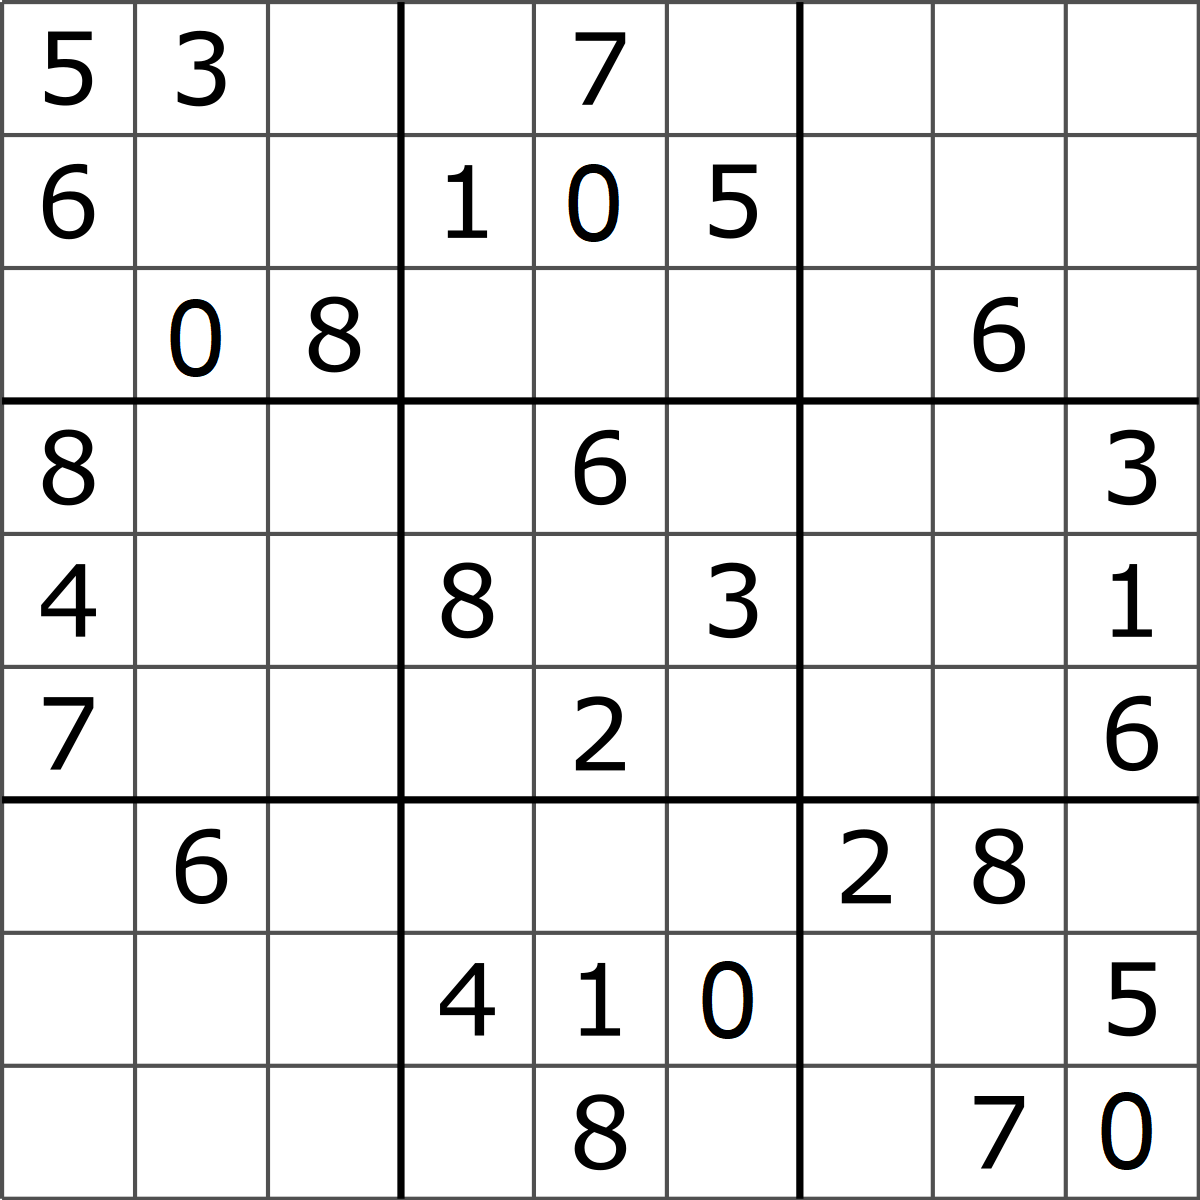
\includegraphics[width=2in]{sample_9_by_9.png}}
				\end{center}
				\caption{An Example Sudoku Board}
			\end{wrapfigure}
			Sudoku is a numerical combinatorial puzzle game. Given a 2 dimensional square grid, the solver is asked to find find an arrangement of numbers that satisfy a specific set of constraints. Here are the set of constraints defined below:	
			\begin{enumerate}
				\item Each cell must contain only one number.
				\item Each row of cells may not have a repeating number.
				\item Each column of cells may not have a repeating number.
				\item Each sub-grid is may not have a repeating number.
			\end{enumerate}
			In the last constraint, a sub-grid is referring to the smaller sized grid of length $\sqrt{N}$ given that the total length of the board is $N$. For example, a board of size $N=9$ will have a sub-grid of size $3$, as evident in Figure 1 above. The goal is to develop a solver that could solve a board of size $N=25$. Consequently, each cell will contain a single integer ranging between 0 and 24 unlike the example in Figure 1.
		\subsection{Sudoku Board Definition}
			\begin{wrapfigure}{l}{0.5\textwidth}
				\begin{center}
					\centerline{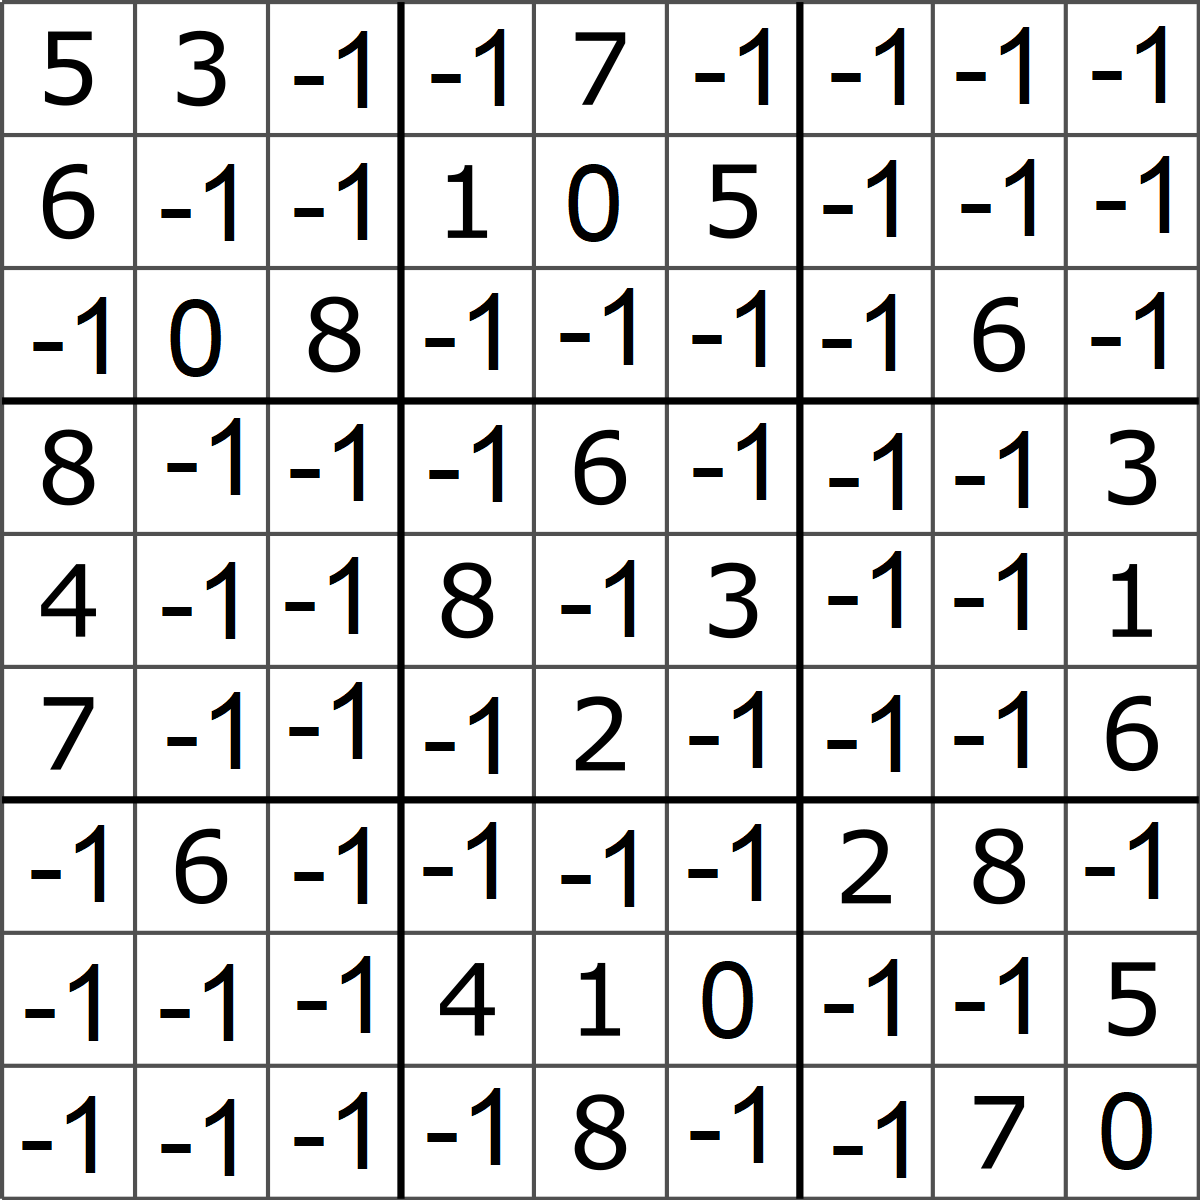
\includegraphics[width=2in]{sample_9_by_9_negative.png}}
				\end{center}
				\caption{Board that the Algorithm Sees}
			\end{wrapfigure}
			To solve this problem, we needed a data structure that could hold all of the information given in the initial board. Therefore, we created a 2 dimensional integer grid with size $N$ by $N$ with every cell filled with an integer from the range $[-1, N)$. Note that $-1$ is included and $N$ is excluded from the possible values. This is because $-1$ represents an empty space on the board, and all the other values represent the numbers that the cell should have. Therefore, instead of the figure above, the algorithm would be seeing a board that look like Figure 2.\\
			A nice property we get from this definition of a Sudoku board is that we get to coordinate each cell with two integers. For example, if we were to get the Figure 1 Sudoku puzzle as an initial board, we can define the first cell with the pair of integers $(1, 0)$ which would have the value $6$.
	\section{Approach}
		Our first observation of the Sudoku problem was that it can be boiled down into constraint satisfaction problem with search. The constraints are the 4 mentioned above, and the searching algorithm is needed because we need to find the correct arrangement of the numbers within a big search space that is the Sudoku puzzle. \\\\
		For example, take a look another look at Figure 1. The cell $(2, 0)$ has the value $-1$, so it needs a value assignment. With all 4 of the constraint applied to the cell, we can see that the only possible values that can take place are $1$ and $2$. With same logic, cell $(1, 2)$ can take the values $2$, $4$, and  $7$. With all these different possibilities, there are different combinations of the number assignment that the board can have. We essentially have narrowed down Sudoku into a problem of finding the specific combination of all the possible combinations of board number assignment.\\\\
		However, this search problem is no easy task. We estimate that there are $N$ possible values that could be assigned to any given cell $(x, y)$, and there are $N^2$ different cells that we need to assign values. Form these assumptions, we can see that the entire search space would be $N^{(N^2)}$. To give it a perspective of a worst case scenario, a mere 9 by 9 board would have $9^{81}$ different possibility, which a 77 digit number. 
	\section{Local Search with Simulated Annealing}
		The first algorithm that we developed to solve Sudoku is a local search method with simulated annealing to introduce randomness. 
		\subsection{Strength and Weaknesses of Local Search}
			A local search method takes a given state, $S$, and modifies is in small increments to find a close neighbor of the given state, $S'$. Then, we can either accept or reject new state $S'$ dependent on whether we find it closer to the goal state. This algorithm is powerful in that it does not require a large space, because at most it needs to remember two states at any given moment. However, a big drawback is that it has the possibility of being stuck in a local extrema.\\\\\
			For example, in the context of the Sudoku board, we might reach a certain point where making any changes will make the board violate more constraints while the current state is not the goal state we are looking for. To combat this problem, we must introduce some randomness to make sure we get away from this local extrema. This is where we use simulated annealing.
		\subsection{Description of Simulated Annealing}
			Simulated Annealing is an optimization technique, inspired by the annealing process used to find a strengthened chemical structure given an initial metal. This is done by carefully and slowly cooling a metal from an immensely high temperature. The 2 properties of this annealing that must be highlighted are the fact that initially the metal is heated and that it is cooled slowly.\\\\
			This idea of temperature management is precisely how we are going to introduce randomness to our local search. At first, we want to introduce the maximum amount of randomness, but as we start to find neighbors that we evaluate to be better, we slowly decrease the randomness causing the problem to zeroing in on a specific solution. The idea is that because we had the freedom to observe many different neighbors of the initial state, we should be able to select the best neighbor.
			\subsubsection{General Outline of the Algorithm}
				Here is the general outline of the local search with simulated annealing algorithm:
				\begin{enumerate}
					\item Initialize the Sudoku board and the temperature
					\item Loop until temperature is at minimum.
						\begin{enumerate}
							\item Loop until maximum number of iterations has been reached.
								\begin{enumerate}
									\item Determine neighboring state via the neighborhood function.
									\item Determine the fitness of the current and neighboring state.
									\item If the neighboring state has a better fitness score than the current, then change the current state to the neighboring state.
									\item Else, if the randomness defined by the temperature permits, change the current state to the neighboring state anyways.
									\item Else stick to the current state.
									\item Keep track of state with lowest energy
								\end{enumerate}
							\item decrease the temperature
						\end{enumerate}
				\end{enumerate} 
			\subsubsection{Initialization}
				The initialization is done by figuring out the frequency of all the values that appear on the initial board and assigning an appropriate amount of each values into all empty cells of the board. For example, in a 9 by 9 board, we want all the values from 0 to 8 to appear exactly 9 times on the board. Ensuring this correctness in  frequency of the values is important, because our switch-value neighborhood function requires it, which is further described below. 
			\subsubsection{Neighborhood Function}
				A neighbor of a given state is determined by randomly choosing two cells that are not initially filled in, and switching the values. Whether a cell was initially filled in or not is evaluated in the initialization step. Because we are changing the values of two cells, we are not introducing a new value to the board in the entirety of the local search process. Therefore, in the initialization step, ensuring the correct frequency of all the values is essential to finding the correct solution.
			\subsubsection{Fitness Function}
				The fitness function implemented here involves determining whether an integer is repeated or is not present in a particular row, column, or the sub-grid. A fitness value is assigned to a possible solution based on the number of repeated or non-present integers. The more repeated or non-present integers there are in a solution's rows, columns, and sub-grid, the higher the fitness value assigned to that solution. Ultimately, the goal state would have a fitness score of 0, because it will not have any repeated or non-present integers.
		\subsection{Evaluation of Local Search with Simulated Annealing}
			In order to evaluate this algorithm, we measure the success rate and total number of iterations given the number of empty cells in the initial Sudoku board. We measure these statistics according to the number of empty cells instead of the actual size of the board, because we hypothesize that the search-space complexity is only dependent on the number of empty cells.\\\\
			For example, a 9 by 9 board has only 81 cells, whereas a 16 by 16 board has 256 cells. However, our neighborhood function only exchanges the values between empty cells, not the entire board. Therefore, if the 9 by 9 board had 50 empty cells and the 16 by 16 board had only 10 empty cells, we should expect that the 16 by 16 board would be solved faster. Therefore, we decided to measure the success rate and the total number of iterations by the total number of empty cells. Here are the results:\\
			\begin{figure}[h]
			\begin{center} 
				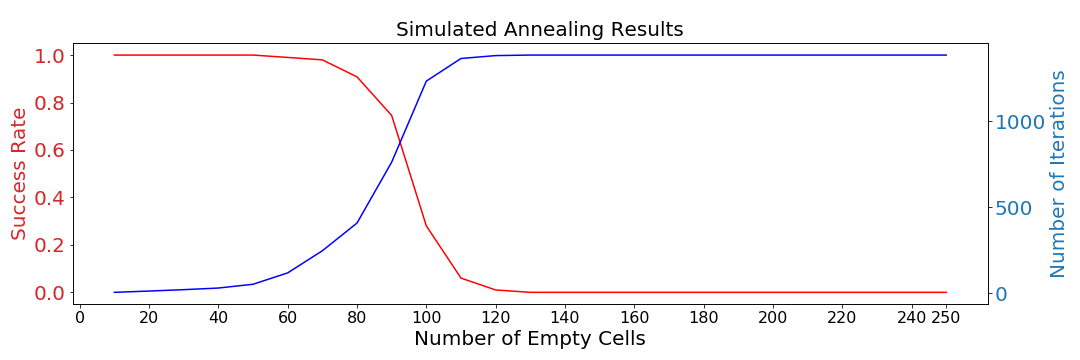
\includegraphics[width=7in]{simulated_annealing_results.png}
				\caption{Success Rate and Number of Iterations for Local Search} 
			\end{center} 
			\end{figure}\\
			It is evident that when there are fewer number of empty cells on the board, which is equivalent to "easy" difficulty, the success rate of the algorithm is nearly $100$\% percent. However, as we increase the number of empty cells, the success rate decreases significantly. At Number of Empty Cells being 120, we nearly have $0\%$ success rate.\\\\
			An explanation for this can be attributed to the fact that our fitness function could be improved. To understand, we analyze a single run's fitness score:\\
			\begin{figure}[h]
				\begin{center} 
					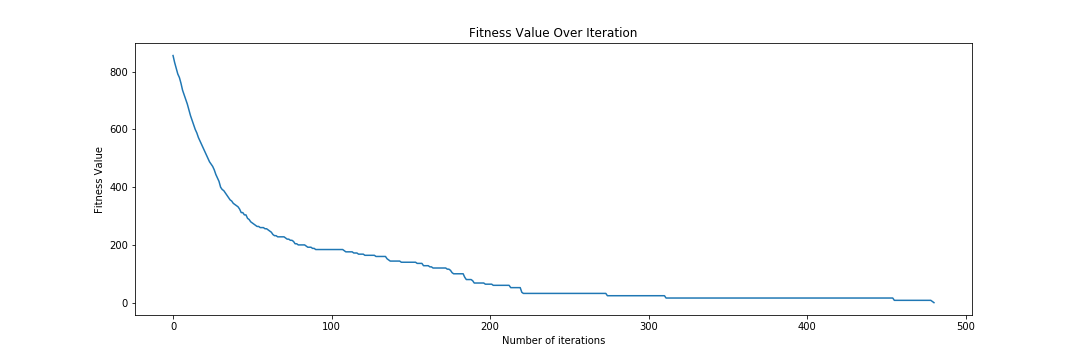
\includegraphics[width=7in]{16_100_iteration.png}
					\caption{Change in Fitness Value over Iterations} 
				\end{center} 
			\end{figure}\\
			Above is a plot of the fitness function for a successful run of a 16 by 16 board with 90 cells empty. We notice a sharp decrease in the early stages of the run, whereas the change in fitness value from $200^{th}$ iteration on-wards is imperceptible. This is where the fitness function fails to quickly identify which neighbors are actually close to the goal state. Once in this phase where the fitness score cannot guide the local search, the search becomes almost random, resulting in failure most of the time.\\\\
			We conclude here that to achieve better results in a scaled up environment with higher difficulty, we need to be able to develop a better fitness function that can distinguish the final few changes that remain at the end of the runs.
	\section{Genetic Algorithm}
		The second algorithm that we implemented is a genetic algorithm. 
		\subsection{Strength and Weaknesses of Genetic Algorithm}
			Genetic algorithm is similar to the above local search with simulated annealing algorithm in that  they are both stochastic search methods. Therefore, we can expect this algorithm to have relatively small space requirements and able to prevent being stuck in a local minima. However, the genetic algorithm differs from the previous algorithm in 2 major ways:
			\begin{enumerate}
				\item Population of candidates instead of a single neighbor
				\item Mutation function instead of neighboring function
			\end{enumerate}
			As you can tell from the word choices, this algorithm is inspired by the process of natural selection. The details of the implementation are explained further below, but overall, this algorithm attempts to introduce an increased amount of variability per iteration by having a group of board configuration instead of having a single individual.
		\subsection{Description of a Population and its Mating Process}
			The goal of this algorithm is to maintain a fixed size of a population of Sudoku board configurations in every generation, while continuously improving the overall "fitness" score. Because every iteration consists of this population, we will refer to them as a generation and a member of a generation as an individual.\\\\
			First, given a generation, we proceed to score every individual in the generation via the fitness function mentioned in the previous section. Secondly, we randomly choose pairs of individuals from the generation to mate and produce the next generation. However, we bias this selection process so that it is more likely to select the individuals with better fitness score more often. Here is the exact outline of the algorithm:
			\subsubsection{General Outline of the Algorithm}
			\subsubsection{Initialization}
			\subsubsection{Mate Selection}
			\subsubsection{Mutation Function}
		\subsection{Evaluation of Genetic Algorithm}
			Similar to the way we evaluated the local search algorithm before, we measure the success rate and the number of generations from the genetic algorithm. Here are the results:
	\section{Backtracking Algorithm}
		Last algorithm that we implemented is a non-stochastic backtracking algorithm with Arc consistency, Minimum Remaining Value ordering (MRV), and Least Constraining Value (LCV) selection.
		\subsection{Strength and Weaknesses of Backtracking Algorithm}
			Backtracking is a way of applying depth-first search to a constraint satisfaction problem. The algorithm selects an empty cell, and tries the possible number assignments that does not violate the above 4 constraints. After making a valid assignment, it proceeds to make more assignments. If at any point the algorithm finds out that for a chosen cell, there are no possible values that preserves the 4 constraints, it will back track the most recent assignment, and it will try a different value in the removed cell. If the algorithm backtracks to the initial state of the board with no possible number assignments left, then the algorithm will return a "fail".\\\\
			Because this algorithm does not have any randomness in its search, it has an amazing property of guaranteeing the absence of solution when it fails. However, the same non-stochastic aspect of the algorithm is its biggest downfall. The run time of the algorithm is slower than the first two algorithms, because in worst case scenario, it has to search through $O(N^{N^2})$ possibilities.
		\subsection{Description of Backtracking Algorithm}
			\subsubsection{General Outline of the Algorithm}
				BacktrackAlgorithm()
				\begin{enumerate}
					\item Order the variable according to MRV
					\item Order the possible number assignments according to LCV
					\item Loop over the ordered number assignments:
					\begin{enumerate}
						\item check if the assignment meets the 4 constraints
						\item If it does not meet the constraints, terminate loop
						\item If it does meet the constraints, Assign the number to the cell
						\item check if the board is Arc consistent
						\item if the board is not Arc consistent, terminate loop
						\item if the board is Arc consistent, call BacktrackAlgorithm()
						\item check result of BacktrackAlgorithm()
						\item if successful/ true, return true
						\item otherwise continue to next iteration of the loop
					\end{enumerate}
					\item return failure/ false
				\end{enumerate}
			\subsubsection{Minimum Remaining Value Order}
				\begin{wrapfigure}{r}{0.5\textwidth}
					\begin{center}
						\raisebox{0pt}[\dimexpr\height-1.0\baselineskip\relax]{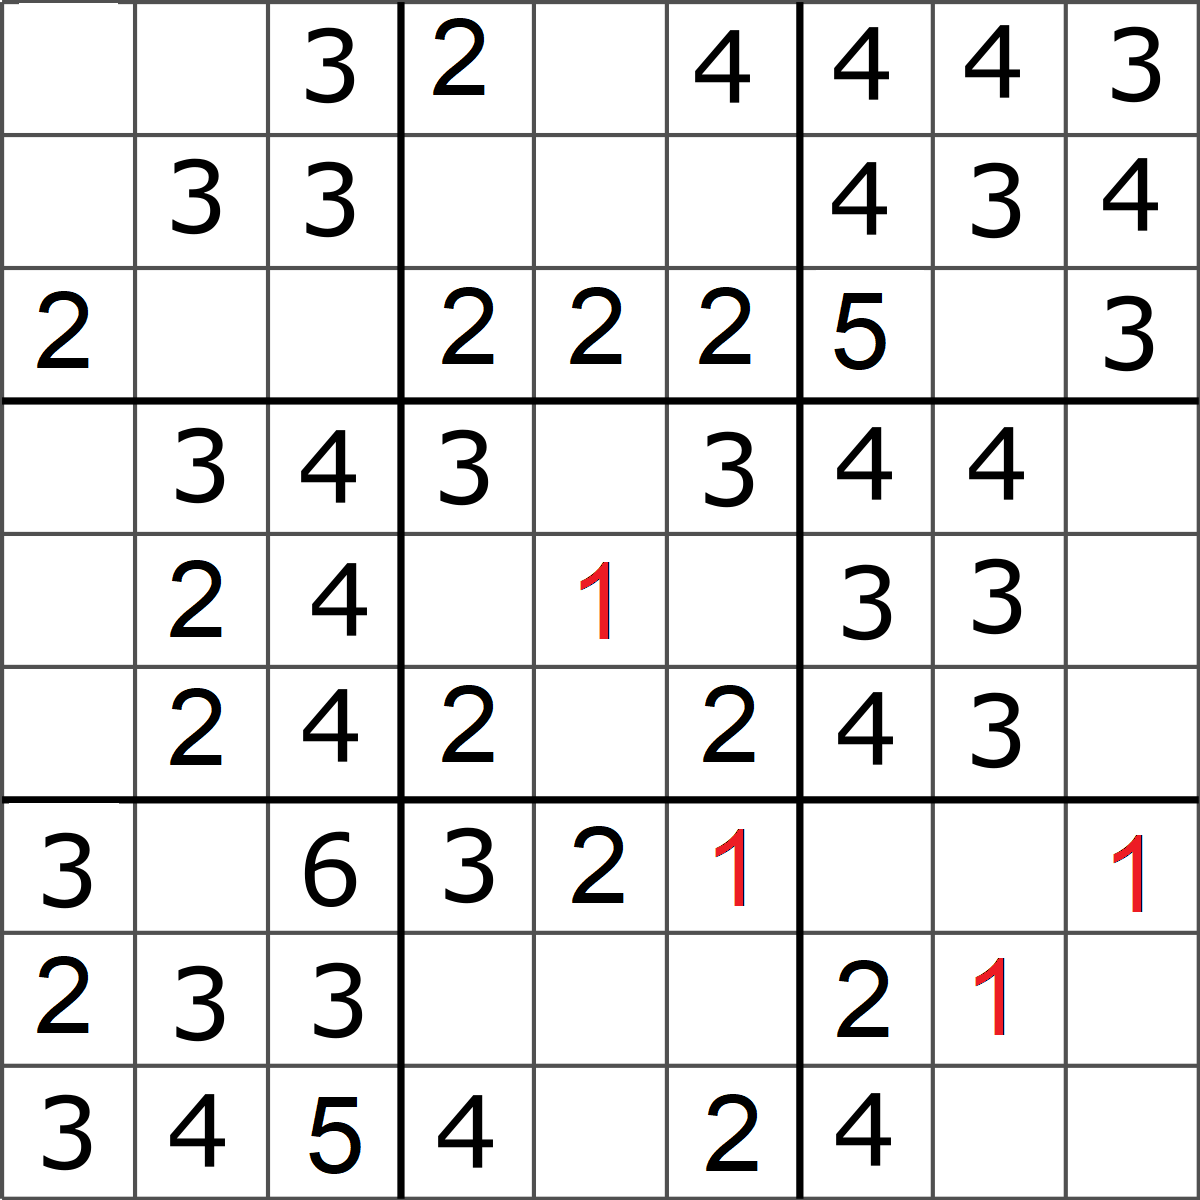
\includegraphics[width=2in]{sample_9_by_9_domain_size.png}}
					\end{center}
					\caption{Possible Domain Sizes}
				\end{wrapfigure}
				When we are choosing which cell to assign a number to, we choose the cell that has the least number of possible values. For example, the from the Figure 1 initial board, we get the Figure 3 as our domain size. Then, our MRV algorithm will choose one from the following set of cells to assign values:
				$$(4, 4), (6, 5), (6, 8), \text{ or } (7, 7)$$
				This because these 4 cells have the least number of possible values. Essentially, MRV algorithm reduces the size of the total space that needs to be searched.\\\\
				Furthermore, when we have ties from the Minimum Remaining Value ordering, we use the Maximum Degree Heuristic to break the ties. This is done by checking how many empty cells it has in its corresponding row, column, and the box. For example, we will choose $(6, 5)$, because it has 14 different empty cells, whereas cells $(4, 4), (6, 8),$ and $(7, 7)$ only have 10, 12, and 11 empty cells respectively.
			\subsubsection{Least Constraining Value Selection}
				After having chosen a cell, we must decide which value to assign. This is determined by the Least Constraining Value selection, which means that we select values that most likely to be correct. This heuristic allows us to arrive at the solution quicker than otherwise.
			\subsubsection{Arc Consistency}
				We implemented AC-3 algorithm outlined in the lecture slides, and it allows us to reduce the search space by eliminating some of the possible choices. In some simple 9 by 9 cases, the solution can be found without a single backtrack.
		\subsection{Evaluation of Backtracking Algorithm}
			In order to evaluate this algorithm, we measure the number of backtracks given the empty cells in a board, and here are the results:
			\begin{figure}[h]
				\begin{center} 
					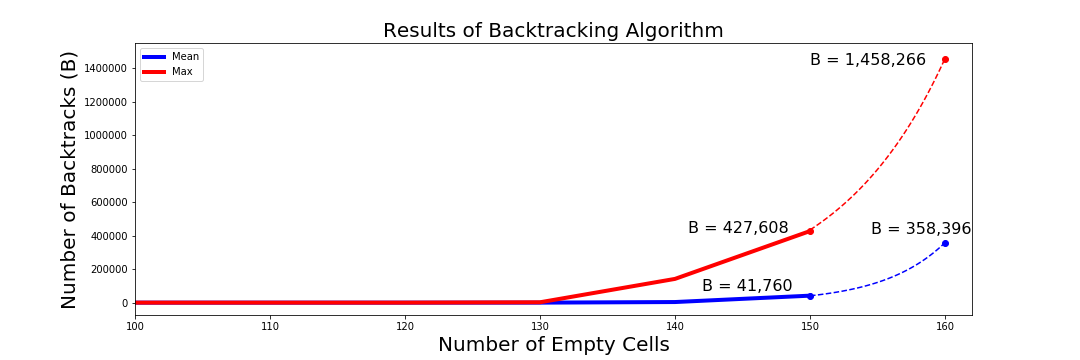
\includegraphics[width=7in]{backtrack.png}
					\caption{Number of Backtracks for Every Difficulty of the Sudoku Board} 
				\end{center} 
			\end{figure}\\
			First thing to notice is that the number of backtracks is nearly 0 up until 130 empty cells. This is because most of these cases the Arc consistency algorithm solves most of the puzzle, and there are no need for any backtracking. However, as soon as the number of empty cells grows beyond 140, the number of backtracking grows exponentially. At 150 empty cells, the backtracking algorithm nearly takes on average about $41,000$ backtracks. This is equivalent to 2 minutes depended on the clock cycle speed of the environment. At this rate, at 160 cells removed, the algorithm is expected to take over 300,000 backtracks which takes about 20 minutes. When considering the worst case scenario, the algorithm could take over a million backtracks, which would take about an hour and 15 minutes.\\\\
			Although backtracking algorithm performs better than local search with simulated annealing, backtracking algorithm fails to scale up to the difficulty of the Sudoku puzzle we want to solve. Our goal is a 25 by 25 board which can have up to 625 cells empty. We expect that developing a better heuristic might be able to improve the algorithm slightly, but the ability to scale up to 600+ empty cells seems implausible for backtracking algorithm.
	\section{Conclusion}
\end{document}